\newpage
\section{Snowflakes}

In this activity, we're going to create snowflakes using the rep-tiles from Activity A11.  Instead of using rep-tiles to make larger versions of the same shape, we'll divide the rep-tile into smaller, similar copies of itself.

We'll do this for a rep-4-tile, but there's nothing special going on with the number 4.  Here are the steps to follow:
\begin{enumerate}
	\item Divide each copy of your rep-4-tile into four smaller, similar copies.
	\item Choose one of the four copies.  (Choose the same copy every time.)
	\item Remove this copy from your shape.  (For now, just shade it in.)
\end{enumerate}
  Each repeat of these steps is called an ``iteration''.
  
If we could do infinitely many iterations, the result would be a \textit{fractal}.\index{fractal}  What kind of symmetry does a fractal have?


\break

\begin{prob}
Here is a triangle.  We've seen that it is a rep-4-tile.  Complete four iterations on this shape.
\[
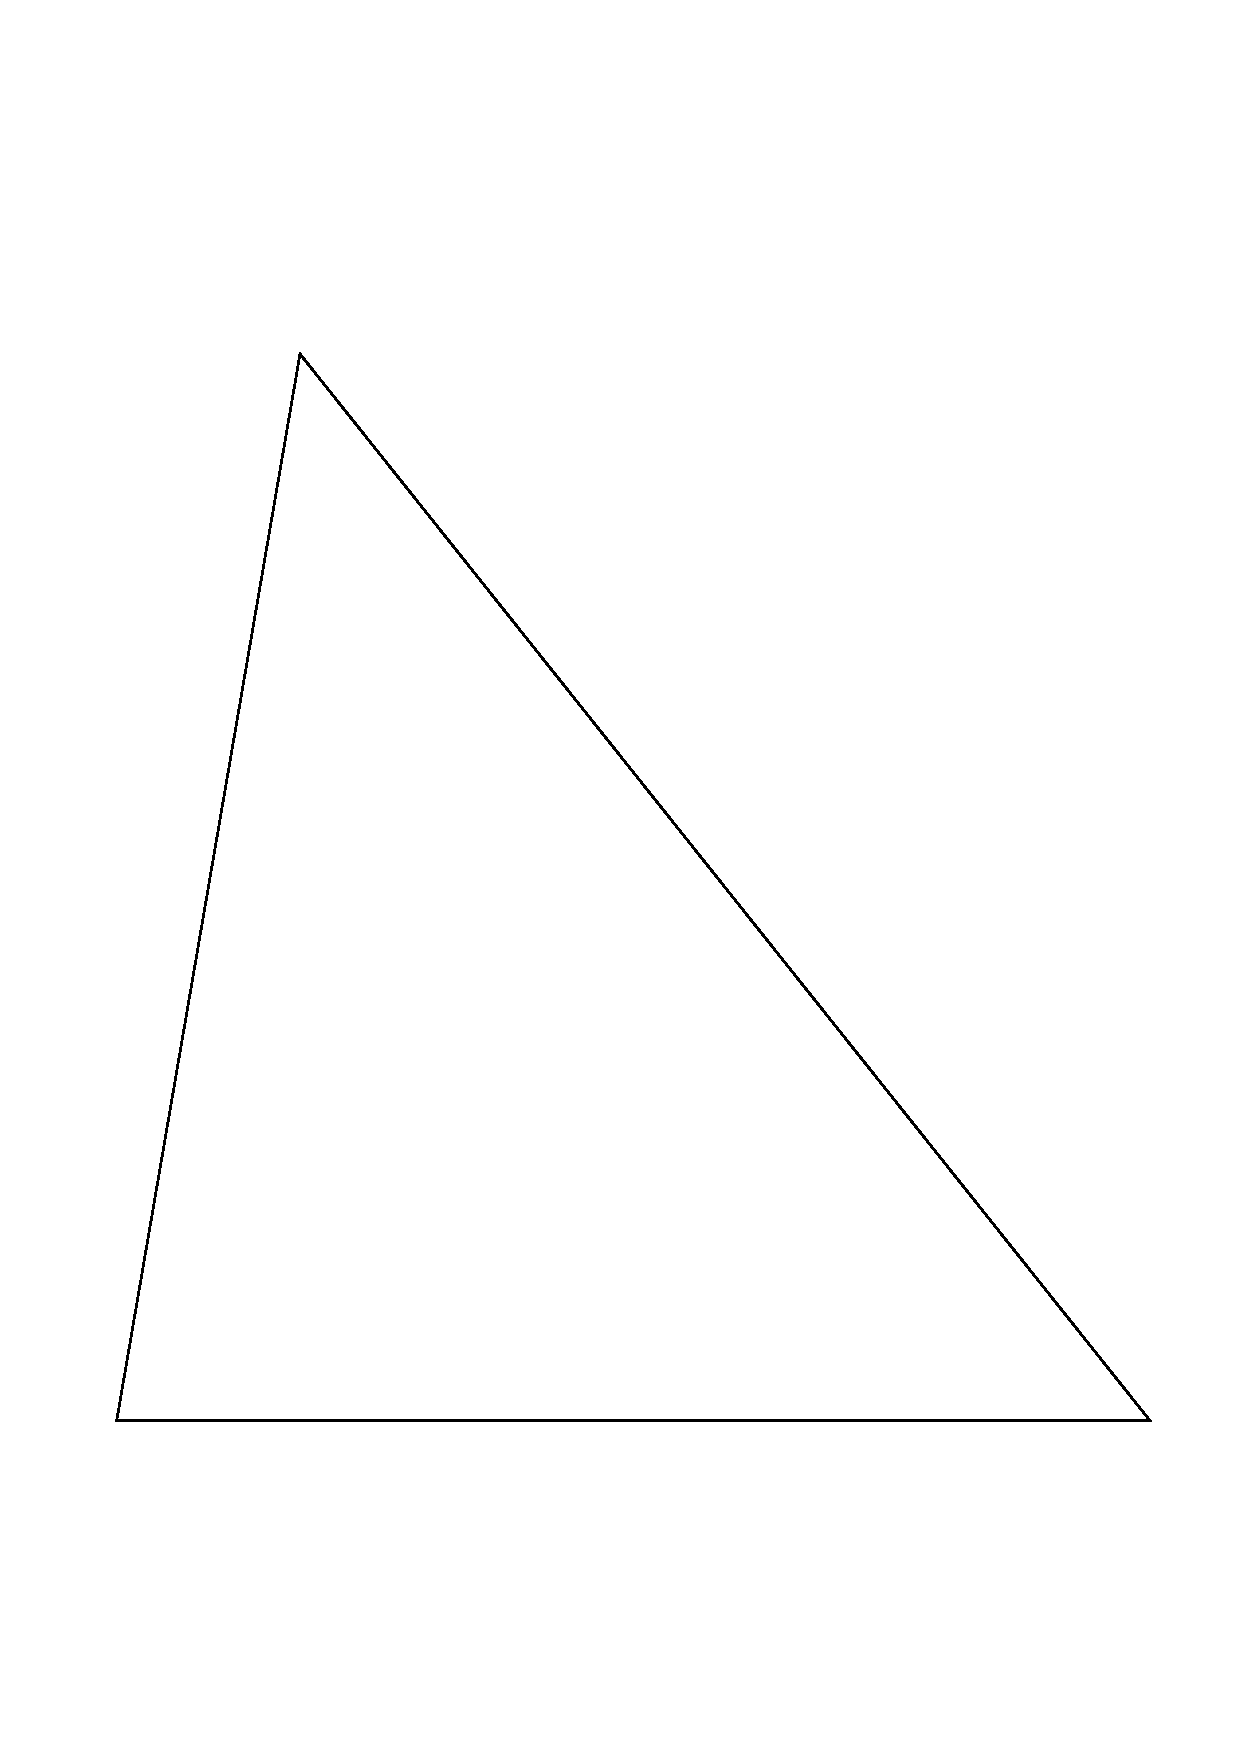
\includegraphics[scale=0.65]{../graphics/snowflake-tri.pdf}
\]

\end{prob}

\break

\begin{prob}
Here is a rep-4-tile called the Sphinx.  As a gesture of friendship, I've done the first iteration for you.  Continue the process by doing three more iterations.
\[
  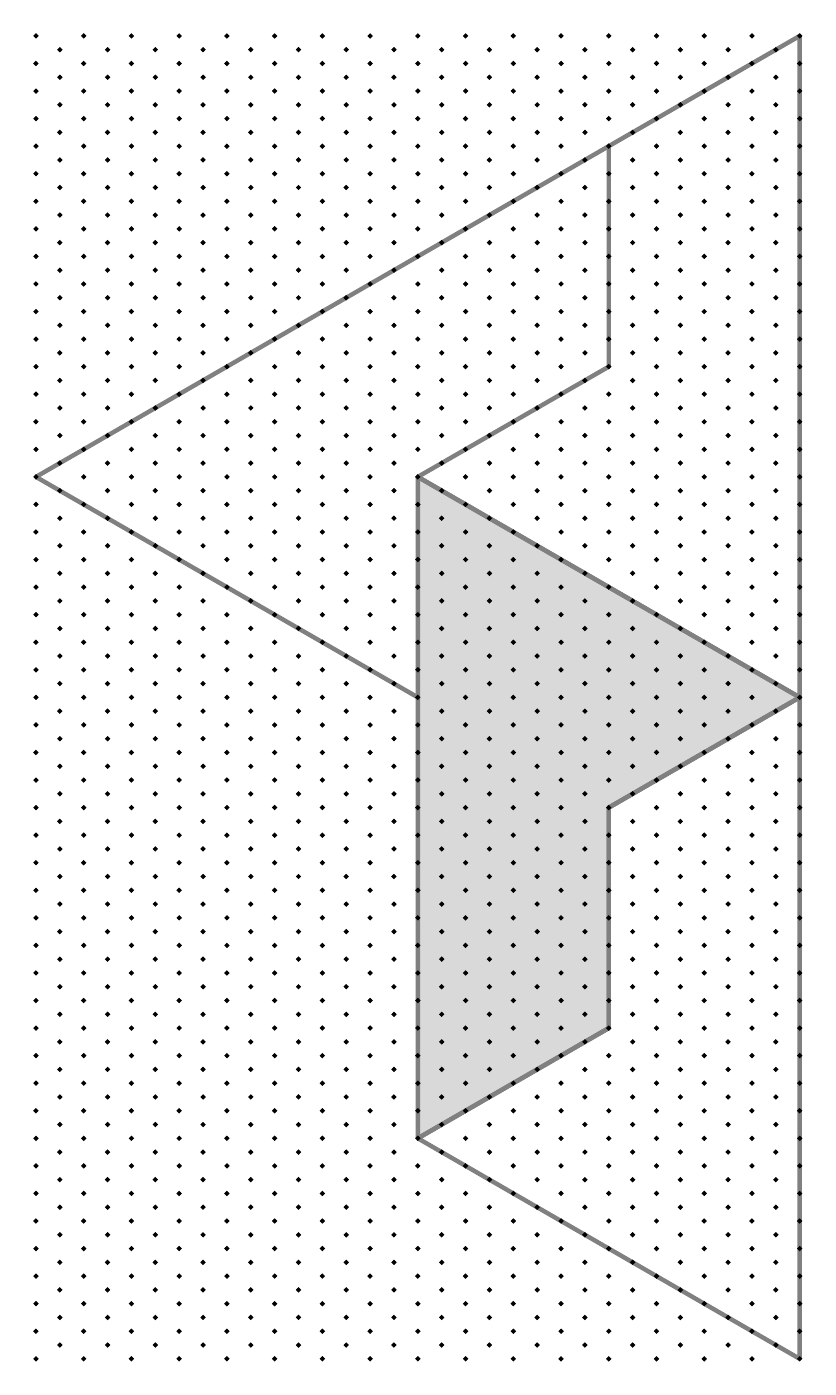
\begin{tikzpicture}[scale=0.35,rotate=90]%% adopted from http://www.texample.net/tikz/examples/lattice-points/
    \clip (-.3,-.3) rectangle (48+.3,{32*sqrt(3)/2+.3}); % Clips the picture...
    %\pgftransformcm{sqrt(3)/2}{.5}{0}{1}{\pgfpoint{0cm}{0cm}}
    \pgftransformcm{1}{0}{.5}{sqrt(3)/2}{\pgfpoint{0cm}{0cm}}
    \filldraw[fill=gray, fill opacity=0.3, draw=gray,ultra thick,line join=bevel] (0,16) -- (24,16) -- (24,0) -- (16,8) -- (8,8) -- cycle;
    \draw[ultra thick, gray,line join=bevel]  (0,0) --    (24,0) -- (16, 8) -- (8,8) -- (0,16) -- cycle;
    \draw[ultra thick, gray,line join=bevel] (24,0) -- (48,0) -- (40, 8)-- (32,8) -- (24,16) -- cycle;
    \draw[ultra thick, gray,line join=bevel] (40,8) -- (16,32) -- (16,16);% -- (24,0);
          
    \foreach \x in {-16,-15,...,48}{% Two indices running over each
      \foreach \y in {0,1,...,32}{% node on the grid we have drawn 
        \node[draw,circle,inner sep=.5pt,fill] at (\x,\y) {};
            % Places a dot at those points
      }
    }
              \end{tikzpicture}
              \]
%% \[
%% 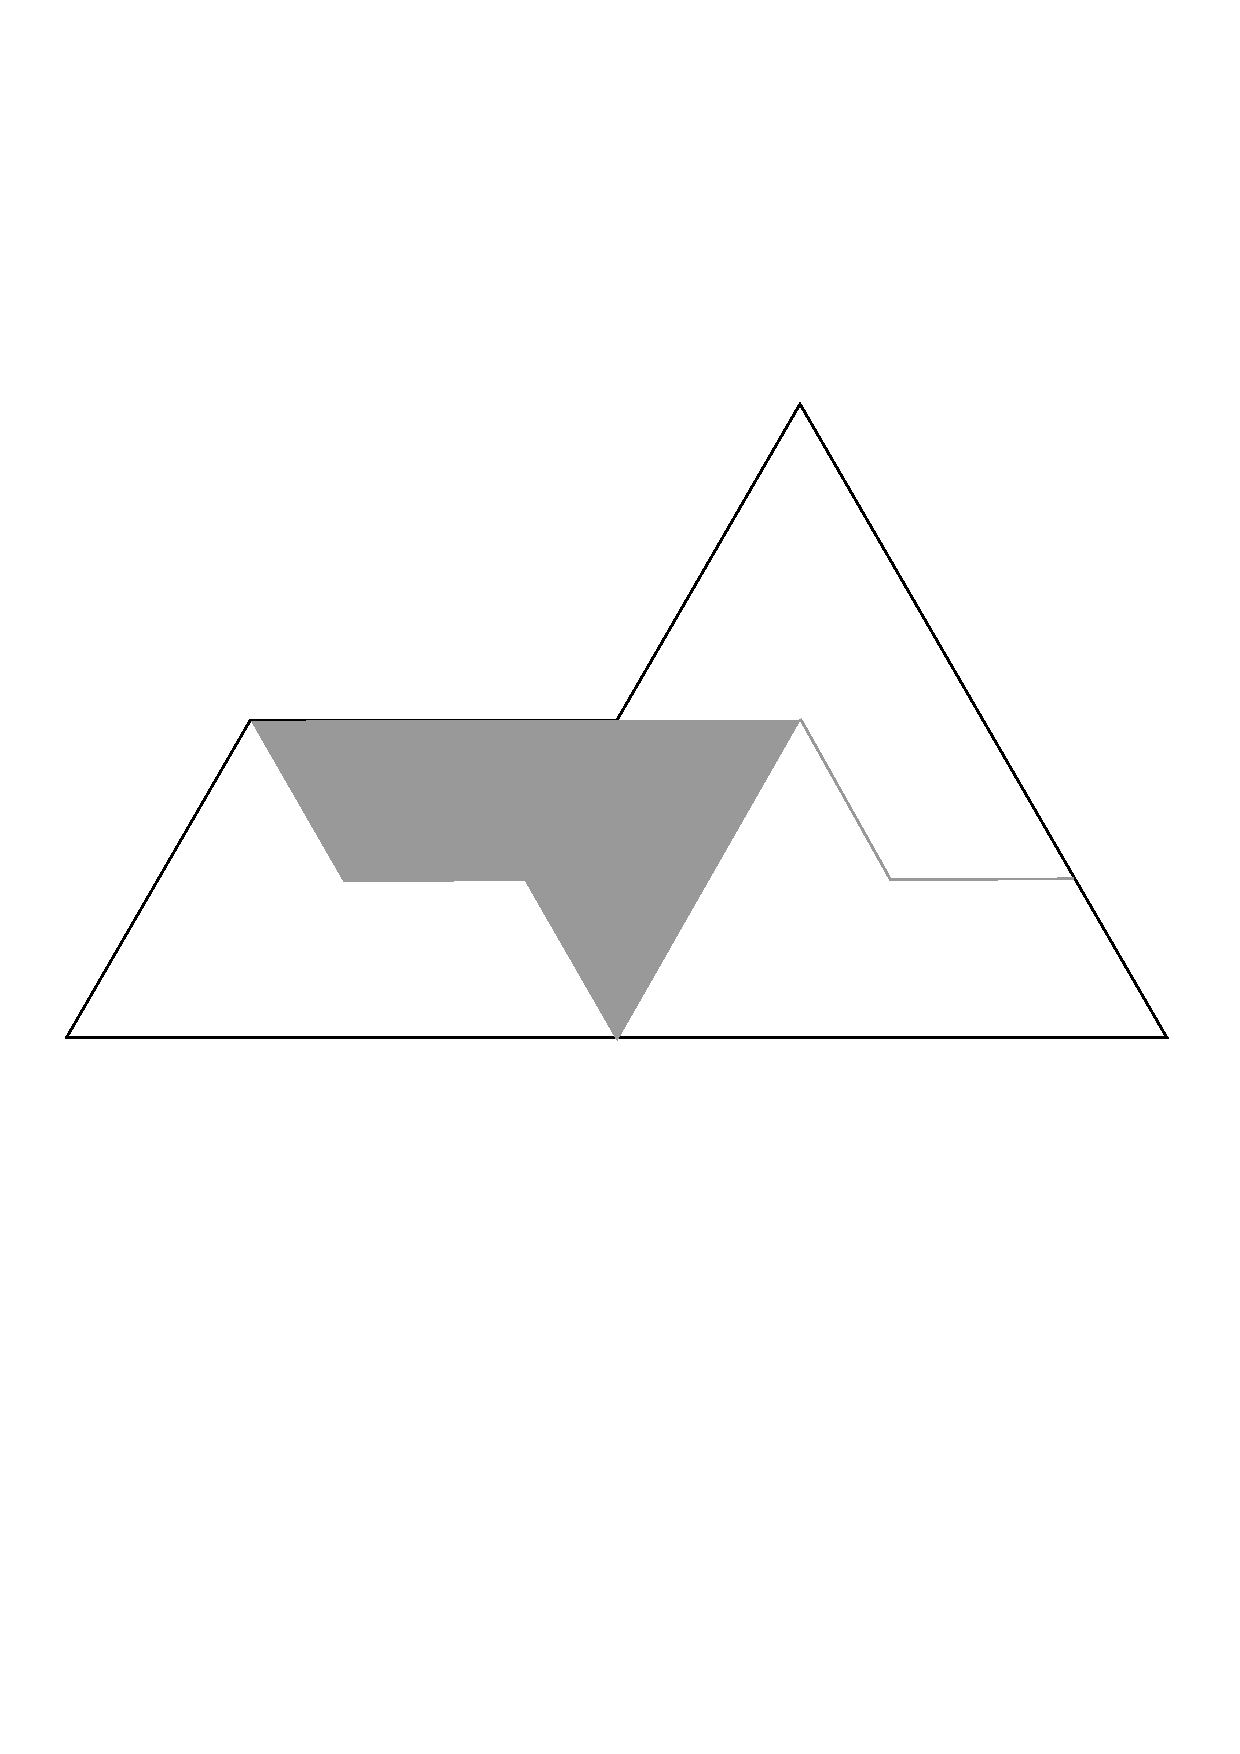
\includegraphics[scale=0.65]{../graphics/snowflake-sphinx.pdf}
%% \]
\end{prob}

\begin{prob}  Suppose the area of the original Sphinx is $A$.  What is the area after the first iteration?  The second iteration?
\end{prob}

\begin{prob}
 If we could do infinitely many iterations, what would the resulting area be?
\end{prob}

\begin{prob}
 We can think of the Sphinx as constructed from 6 equilateral triangles.  (Draw it!)  If the side length of each triangle is four, what is the perimeter of the Sphinx?
 \end{prob}

\begin{prob}
 Calculate the new perimeter after the first, second, and third iterations.
 \end{prob}

\begin{prob}
  If we could do infinitely many iterations, what would the perimeter be?
  \end{prob}

